\documentclass[conference]{IEEEtran}

\usepackage[T1]{fontenc}
\usepackage[utf8]{inputenc}
\usepackage{amsmath}
\usepackage{amssymb}
\usepackage{booktabs}
\usepackage{graphicx}
\usepackage{microtype}
\usepackage{tikz}
\usepackage{url}
\usepackage{xurl}
\usepackage[hidelinks]{hyperref}
\usetikzlibrary{arrows.meta,fit,positioning}

\definecolor{deedyred}{RGB}{177,52,52}
\definecolor{deedyorange}{RGB}{196,111,21}
\definecolor{deedyblue}{RGB}{42,96,153}
\definecolor{deedygreen}{RGB}{48,126,91}
\tikzset{
    deedybox/.style={draw, rounded corners=2pt, align=center,
        minimum height=8mm, inner sep=4pt, fill=white},
    deedyarrow/.style={-{Latex[length=2mm]}, semithick},
    deedydashed/.style={-{Latex[length=2mm]}, semithick, dashed}
}

\setlength{\textfloatsep}{9pt plus 2pt minus 2pt}
\setlength{\dbltextfloatsep}{9pt plus 2pt minus 2pt}

\title{DEEDY: A Thai-Centric Multi-Agent Framework for\\
Social-Media Marketing Campaign Analysis}

\author{\IEEEauthorblockN{Sawit Koseeyaumporn}
\IEEEauthorblockA{Department of Computer Engineering\\
King Mongkut's University of Technology Thonburi, Bangkok, Thailand\\
\texttt{sawit.kosee@kmutt.ac.th}}}

\begin{document}
\maketitle

\begin{abstract}
Social-media marketing campaigns generate large volumes of fast-moving,
context-dependent consumer reactions that are difficult to interpret with
sentiment classification alone. This paper presents DEEDY (Digital Environment
for Emergent Dynamics and Yield), a Thai-centric application and experimental
testbed for analyzing campaign response with large-language-model (LLM)
agents. For each campaign post, an Apify-based pipeline requests up to 1,000
publicly accessible comments from Facebook, Instagram, or TikTok, preserves
post and collection provenance, and produces synchronized raw and Thai-aware
analysis views. Campaign facts and approved context form a reality seed,
whereas observed reactions reserved for evaluation remain hidden from the
agents. DEEDY adapts MiroFish, an open-source multi-agent prediction engine
that converts seed documents into a GraphRAG-grounded world, generates actors,
runs OASIS social interactions, and supports report generation and post-run
inspection. The resulting application lets marketers examine how message
framing, audience composition, and platform mechanisms may shape simulated
reaction, diffusion, and narrative formation. We propose leakage-resistant
evaluation against held-out Thai comments using sentiment and stance
distribution distance, narrative coverage, response diversity, propagation
error, repeated runs, and native-Thai human assessment. OpenRouter generation
completed 1,300 calls across DeepSeek V4 Flash 0731 and Qwen3 8B. An independent
GLM-5.3-Flash judge then completed 1,482 blinded orientations over 741
real--synthetic pairs. It preferred the authentic comment in 59.3\% of
judgments, although synthetic reactions received higher mean naturalness and
campaign-relevance scores. The results therefore establish neither behavioral
fidelity nor a message-clarity advantage. DEEDY is positioned as an exploratory
campaign-planning and social-listening instrument, not as a deterministic
forecast of consumer behavior or a replacement for field research.
\end{abstract}

\begin{IEEEkeywords}
LLM agents, social-media marketing, campaign analysis, social simulation, Thai
NLP, GraphRAG, MiroFish, Apify
\end{IEEEkeywords}

\section{Introduction}

Marketing campaigns on social media are not one-way messages. Consumers reply
to a campaign post, react to one another, repeat or contest emerging claims,
and carry interpretations across platform feeds. A favorable first response
may be displaced by complaints about price, product quality, brand conduct, or
the credibility of an influencer; conversely, a small positive narrative may
grow through recommendation and peer endorsement. Counting likes or assigning
sentiment to comments can summarize a snapshot, but it cannot by itself
represent the interaction process through which campaign narratives emerge.
Agent-based modeling (ABM) provides a bottom-up way to represent local exposure
and response decisions and observe their collective consequences
~\cite{macal2010tutorial}.

LLM agents extend ABM by allowing simulated actors to condition open-ended
actions on a profile, memory, retrieved evidence, feed context, and earlier
conversation. Generative Agents demonstrated memory-driven believable
behavior~\cite{park2023generative}, while Social Simulacra showed how generated
users and conversations can support social-computing prototypes
~\cite{park2022social}. Systems including $S^3$, OASIS, and GenSim subsequently
modeled social networks, recommendation, and multiple online actions at larger
scales~\cite{gao2023s3,yang2024oasis,tang2025gensim}. These capabilities suggest
a campaign-analysis application in which marketers can rehearse alternative
message framing, audience composition, and feed conditions before interpreting
the resulting differences as hypotheses for further testing.

\textbf{MiroFish} provides the application foundation for this work. The
open-source project describes itself as a multi-agent prediction engine that
constructs a parallel digital world from real-world seed material such as
news, policy drafts, or analysis reports~\cite{mirofish2026}. Its workflow has
five stages: graph building with seed extraction and GraphRAG memory injection;
environment setup with entity, persona, and agent construction; dual-platform
social simulation with temporal memory updates; report generation; and deep
interaction with individual agents or the report agent. OASIS supplies the
underlying social-simulation engine. MiroFish therefore offers a useful bridge
from campaign documents to an inspectable simulated environment, but its
outputs must still be validated before they are used to support marketing
decisions.

Applying this workflow to Thai campaigns introduces two challenges. First,
Thai localization is more than translating an English prompt. Thai has no
obligatory whitespace between words, and campaign comments frequently combine
informal spelling, repeated characters, emoji, hashtags, transliterated
English, regional language, sarcasm, indirect disagreement, and culturally
specific politeness. Thai NLP resources and models have improved substantially
~\cite{arreerard2022survey,phatthiyaphaibun2023pythainlp,
lowphansirikul2021wangchanberta,pipatanakul2024typhoon2}, but cultural capability
remains a distinct evaluation target~\cite{kim2025thaicli}. Second, social data
collection is platform-dependent and incomplete. A reproducible study must
record which campaign post was queried, the collection time, the requested
limit, the returned count, and any access or visibility limitation.

A further methodological problem is that plausible campaign comments do not
prove behavioral fidelity. Demographically conditioned LLM samples can
approximate some human distributions~\cite{argyle2023out}, yet recent work finds
behavioral inconsistency across settings~\cite{mooney2025coherent}. Operational
validation against authentic comments also shows that matching surface form
can be separated from matching content~\cite{schwager2026conditioned}. For this
reason, campaign context needed to construct the simulation must be separated
from real consumer reactions used to test it, and stochastic conditions must
be repeated rather than judged from a single persuasive-looking run.

This paper presents \textbf{DEEDY}, a Thai-centric campaign-analysis
application that combines an Apify data-preparation pipeline, the DEEDY
Simulation Core, and an explicit validation layer. Analysts provide campaign
topics and public post URLs from Facebook, Instagram, or TikTok. DEEDY requests
up to 1,000 comments for each post, preserves provenance and conversation
structure, and separates campaign context from held-out consumer reactions.
Within the simulator, an analyst can compare a baseline campaign with
counterfactual message framing, actor composition, network structure, or
recommendation policy. The application reports where simulated and observed
discourse agree or diverge; it does not claim to forecast the choices of a
specific person or the Thai market as a whole.

Our contributions are threefold:
\begin{itemize}
    \item We define an end-to-end Thai campaign-data pipeline that uses Apify
    Actors to request up to 1,000 publicly accessible comments per campaign
    post, normalize cross-platform fields, preserve provenance, and produce
    Thai-aware views for analysis and simulation.
    \item We adapt the MiroFish/OASIS workflow to social-media marketing through
    campaign-grounded actor construction, Thai linguistic attributes,
    configurable campaign interventions, and auditable simulation outputs.
    \item We specify a leakage-resistant protocol that evaluates content,
    population, and dynamic correspondence against held-out Thai campaign
    reactions using repeated runs, native-Thai review, ablations, and
    uncertainty reporting.
\end{itemize}

\section{Related Work}

Generative Agents introduced memory, reflection, and planning for believable
behavior~\cite{park2023generative}; $S^3$, OASIS, and GenSim extended this idea
to networked social environments, multiple online actions, and reusable
simulations~\cite{gao2023s3,yang2024oasis,tang2025gensim}. MiroFish connects a
reality seed to graph-grounded personas, social simulation, and report
generation~\cite{mirofish2026}. DEEDY adapts this workflow to Thai campaign
analysis and adds an explicit separation between evidence used to construct a
scenario and evidence used to evaluate it.

This separation is important because plausible language is not equivalent to
behavioral validity. Algorithmic fidelity compares generated and human
population distributions~\cite{argyle2023out}, while conditioned-comment
prediction directly compares generated and authentic responses to the same
stimulus~\cite{schwager2026conditioned}. Generative ABMs should therefore be
validated incrementally before counterfactual claims are made
~\cite{cross2025validating}.

Thai social-media analysis adds informal spelling, code-mixing, emoji,
sarcasm, indirect stance, and culturally specific politeness. Thai NLP tools
and pretrained models provide useful linguistic infrastructure
~\cite{arreerard2022survey,phatthiyaphaibun2023pythainlp,
lowphansirikul2021wangchanberta,pipatanakul2024typhoon2}, but cultural knowledge
remains a separate capability~\cite{kim2025thaicli}. Conversation context is
also necessary because sarcasm can reverse literal polarity
~\cite{hazarika2018cascade}. These findings motivate evaluation of naturalness,
cultural fit, stance, and authenticity rather than sentiment alone.

\section{DEEDY System Architecture and Workflow}

\begin{figure*}[t]
    \centering
    \resizebox{0.98\textwidth}{!}{%
    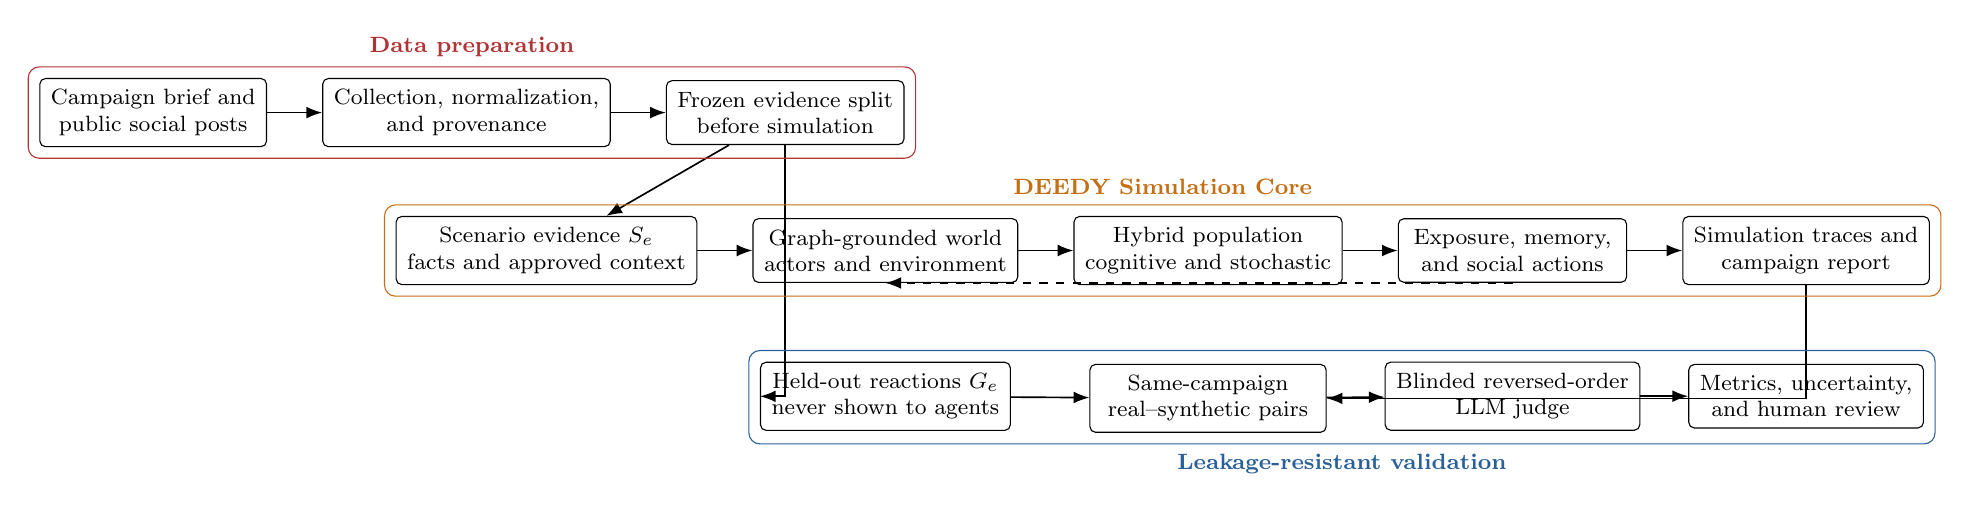
\begin{tikzpicture}[font=\footnotesize, node distance=6mm and 7mm]
        \node[deedybox, minimum width=27mm] (source)
            {Campaign brief and\\public social posts};
        \node[deedybox, minimum width=27mm, right=of source] (corpus)
            {Collection, normalization,\\and provenance};
        \node[deedybox, minimum width=26mm, right=of corpus] (split)
            {Frozen evidence split\\before simulation};

        \node[deedybox, minimum width=29mm, below left=9mm and -4mm of split]
            (scenario) {Scenario evidence $S_e$\\facts and approved context};
        \node[deedybox, minimum width=30mm, right=of scenario] (graph)
            {Graph-grounded world\\actors and environment};
        \node[deedybox, minimum width=30mm, right=of graph] (agents)
            {Hybrid population\\cognitive and stochastic};
        \node[deedybox, minimum width=29mm, right=of agents] (social)
            {Exposure, memory,\\and social actions};
        \node[deedybox, minimum width=28mm, right=of social] (report)
            {Simulation traces and\\campaign report};

        \node[deedybox, minimum width=29mm, below=10mm of graph] (holdout)
            {Held-out reactions $G_e$\\never shown to agents};
        \node[deedybox, minimum width=30mm, below=10mm of agents] (pair)
            {Same-campaign\\real--synthetic pairs};
        \node[deedybox, minimum width=29mm, below=10mm of social] (judge)
            {Blinded reversed-order\\LLM judge};
        \node[deedybox, minimum width=28mm, below=10mm of report] (metrics)
            {Metrics, uncertainty,\\and human review};

        \draw[deedyarrow] (source) -- (corpus);
        \draw[deedyarrow] (corpus) -- (split);
        \draw[deedyarrow] (split) -- (scenario);
        \draw[deedyarrow] (split) |- (holdout);
        \draw[deedyarrow] (scenario) -- (graph);
        \draw[deedyarrow] (graph) -- (agents);
        \draw[deedyarrow] (agents) -- (social);
        \draw[deedyarrow] (social) -- (report);
        \draw[deedydashed] (social.south) |- (graph.south);
        \draw[deedyarrow] (holdout) -- (pair);
        \draw[deedyarrow] (report) |- (pair);
        \draw[deedyarrow] (pair) -- (judge);
        \draw[deedyarrow] (judge) -- (metrics);

        \node[draw=deedyred, rounded corners=4pt,
            fit=(source)(corpus)(split), inner sep=4pt,
            label={[text=deedyred,font=\bfseries\footnotesize]above:Data preparation}] {};
        \node[draw=deedyorange, rounded corners=4pt,
            fit=(scenario)(graph)(agents)(social)(report), inner sep=4pt,
            label={[text=deedyorange,font=\bfseries\footnotesize]above:DEEDY Simulation Core}] {};
        \node[draw=deedyblue, rounded corners=4pt,
            fit=(holdout)(pair)(judge)(metrics), inner sep=4pt,
            label={[text=deedyblue,font=\bfseries\footnotesize]below:Leakage-resistant validation}] {};
    \end{tikzpicture}%
    }
    \caption{DEEDY architecture and executed evaluation workflow. Campaign
    facts construct the simulated world, while authentic reactions remain
    hidden until outputs are scored. The dashed arrow represents memory
    feedback within the simulation.}
    \label{fig:deedy-architecture}
\end{figure*}

\subsection{Evidence Preparation}

Public campaign posts and comments are collected from Facebook, Instagram,
and TikTok through recorded Apify queries~\cite{apify2026actors}. Text is
preserved with emoji, Thai--English code-mixing, repeated characters, and
thread cues because these may carry pragmatic meaning. Direct identifiers are
removed from research views, while campaign, platform, post, time, and
collection provenance are retained. The resulting corpus is not treated as a
random sample of Thai consumers: platform visibility, ranking, moderation,
deletion, and source selection can affect which comments are observable.

For campaign $e$, evidence is partitioned before generation as
\begin{equation}
    D_e=S_e\;\dot\cup\;G_e,
\end{equation}
where $S_e$ contains only facts and context permitted to construct the
scenario, and $G_e$ contains authentic reactions reserved for evaluation.
Comments, their summaries, and derived sentiment proportions from $G_e$ are
not supplied to agents. This design prevents the simulator from repeating the
answers against which it will later be scored.

\subsection{DEEDY Simulation Core}

Figure~\ref{fig:deedy-architecture} presents the conceptual architecture. The
deployed component is called the \emph{DEEDY Simulation Core}; MiroFish is the
underlying engine. Its hybrid-agent and dual-memory design is informed by the
ISAL-NLP architecture~\cite{marketfish2026architecture}. First, campaign facts
are converted into a graph-grounded world containing entities, relations, and
retrievable memories. Audience roles are then sampled with interests, prior
attitudes, activity, language register, and uncertainty. Unsupported details
remain explicit assumptions rather than facts.

The population combines a smaller cognitive tier with a larger stochastic
tier. Cognitive agents retrieve relevant memories, observe a bounded feed,
update their private stance, and generate a Thai action or remain silent.
Stochastic agents preserve population scale using a probabilistic response
conditioned on prior attitude, exposure, neighbors, and the preceding social
signal. For an exposed stochastic agent $i$ at time $t$,
\begin{equation}
 \Pr(a_{i,t}\!\ne\!\varnothing)=\sigma(\beta_0+\beta_b b_i+
 \boldsymbol{\beta}_d^\top\mathbf d_i+\beta_s s_{t-1}+\beta_x x_{i,t}).
\end{equation}
The action space includes like, share, comment, reply, and silence. Initial
exposure can be chronological, interest-based, popularity-based, or seeded
through influential agents; later exposure propagates through the configured
network. These mechanisms are experimental assumptions, not reconstructions
of a platform's proprietary recommender.

Short-term memory stores current exposures and interactions, while long-term
retrieval preserves scenario knowledge and reflected experience. Every output
connects an action to its actor, exposure, retrieved evidence, parent action,
and simulated time. The final report summarizes sentiment, stance, narratives,
reach, engagement, influential actors, and disagreement across repeated runs.
This traceability supports error analysis and counterfactual comparison but
does not make a simulated difference a real-world causal effect.

\section{Evaluation and Experimental Results}

\subsection{Data and Experimental Design}

The evaluation covers five Thai campaigns: Parameter Gelato, KFC Bucket Ware,
MK Buffet, Walk/Run for Glasses by Top Charoen, and Thai Chuai Thai Plus. The
corpus contains 5,000 authentic comments from 33 posts, with 1,000 comments per
campaign. Aggregate sentiment analyses were used only after generation. The
available crawl contained no reply links, so observed cascade correspondence
could not be evaluated; network results are reported only as model
sensitivity.

Experiments~1--3 test grounding, Thai prompting, and the response model.
Experiment~4 varies feed and network assumptions and generates agent reactions.
Experiment~5 compares a baseline campaign packet with a clarity frame that
makes conditions and uncertainties more explicit. Ten random seeds are used
per campaign-condition combination. Jensen--Shannon distance (JSD) measures
sentiment-distribution divergence, while text quality is assessed with
diversity, semantic correspondence~\cite{zhang2020bertscore}, and blinded
judgment. Table~\ref{tab:experiments-compact} reports only the conclusions
supported by the executed pilot.

\begin{table*}[t]
\caption{Executed experiments and essential findings. JSD comparisons use the
available aggregate reference and are diagnostics rather than held-out causal
estimates.}
\label{tab:experiments-compact}
\centering
\footnotesize
\begin{tabular}{@{}p{0.08\textwidth}p{0.24\textwidth}p{0.58\textwidth}@{}}
\toprule
Experiment & Comparison & Essential result \\
\midrule
1 & Grounded vs. ungrounded generation & Paired JSD intervals spanned zero for
both generators; grounding did not establish a fidelity advantage. \\
2 & Thai-context vs. translated or normalized prompts & JSD intervals spanned
zero. Thai-script frequency was high but cannot establish naturalness or
cultural competence. \\
3 & Two LLMs vs. stochastic ABM & No pairwise sentiment-JSD interval excluded
zero; the ABM generated states rather than language. \\
4 & Feed and network sensitivity; LLM reaction panel & Results were much more
sensitive to the assumed network than population size. The best LLM-panel mean
JSD was 0.2995, and negative reactions were under-produced. \\
5 & Baseline vs. clarity frame & Across 100 matched generator--campaign--seed
pairs, clarity changed JSD by $-0.0030$ (95\% empirical interval
$-0.1888$--$0.1261$); no reliable advantage was found. \\
\bottomrule
\end{tabular}
\end{table*}

Across Experiments~1--5, 1,300 generation calls completed. Experiments~4--5
produced 6,400 agent records from 800 calls. Of these, 741 calls contained at
least one visible reaction; 59 all-silence calls were retained in action-rate
analysis but excluded from text comparison. The Experiment~4 panel showed only
modest changes across feed/network prompt descriptions: DeepSeek JSD ranged
from 0.2995 to 0.3233 and Qwen from 0.3274 to 0.3432. In the separate
non-generative mechanism sweep, the assumed network produced substantially
larger reach and action-rate changes than population size. Because the corpus
did not preserve reply edges, neither topology can be interpreted as an
observed Thai interaction network.

\subsection{Blinded LLM-as-a-Judge Evaluation}

Each eligible synthetic reaction was paired with a distinct authentic comment
from the same campaign. Direct identifiers and contact patterns were removed;
the judge received only the campaign facts and two unlabeled texts. Each of
the 741 pairs was evaluated twice with A/B order reversed, producing 1,482
valid judgments. GLM-5.3-Flash, accessed through OpenRouter
~\cite{openrouter2026glm53flash}, scored Thai naturalness, campaign relevance,
social-media plausibility, pragmatic/cultural fit, contextual specificity, and
unsupported-claim risk on five-point scales. It also predicted sentiment and
selected which text appeared more authentic. Pair reversal was used because
LLM judges may exhibit presentation and position biases
~\cite{shi2024judging}. Aggregate sentiment references were hidden until all
judgments were complete.

The authentic comment was preferred in 59.3\% of judgments, the synthetic
reaction in 40.6\%, and a tie in 0.1\%. Treating a tie as half a win gives a
synthetic-realism score of 0.406 (bootstrap 95\% CI 0.374--0.438), below the
0.5 indifference point. Reversed-order preference agreed for 83.5\% of pairs,
while candidate A was selected in 55.9\% of non-ties, confirming measurable
position sensitivity.

\begin{table}[t]
\caption{Blinded judge results over 741 real--synthetic pairs. Score gaps are
synthetic minus real; risk is the only dimension where higher is worse.}
\label{tab:judge-results}
\centering
\scriptsize
\begin{tabular}{@{}lrrr@{}}
\toprule
Dimension & Real & Synthetic & Gap (95\% CI) \\
\midrule
Thai naturalness & 3.77 & 4.19 & 0.42 [0.29, 0.57] \\
Campaign relevance & 2.83 & 4.46 & 1.64 [1.51, 1.77] \\
Social plausibility & 3.84 & 3.88 & 0.04 [$-0.11$, 0.20] \\
Cultural fit & 3.57 & 4.07 & 0.50 [0.35, 0.65] \\
Context specificity & 2.23 & 3.14 & 0.91 [0.76, 1.05] \\
Unsupported-claim risk & 1.83 & 1.87 & 0.04 [$-0.06$, 0.14] \\
\bottomrule
\end{tabular}
\end{table}

Table~\ref{tab:judge-results} reveals a useful tension. Synthetic reactions
were rated more natural, relevant, culturally appropriate, and specific, yet
authentic comments were more often selected as real. Social plausibility and
unsupported-claim risk showed no clear difference. The judge-labeled sentiment
distribution diverged less from the aggregate reference for authentic comments
($\mathrm{JSD}=0.077$) than for synthetic reactions ($0.215$), reinforcing the
under-production of negative response. KFC was the only campaign with a
synthetic-realism score slightly above 0.5, whereas Top Charoen had the largest
authenticity gap. Campaign slices are diagnostic because sample eligibility
and judge priors may differ.

\subsection{Campaign-Level Results}

Table~\ref{tab:campaign-results} reports all five campaign slices. The realism
interval exceeded neither the 0.5 indifference point nor its uncertainty for
any campaign. KFC was closest to indifference, while Top Charoen was most
readily distinguished from authentic discussion. Sentiment correspondence did
not always move with authenticity: Top Charoen's synthetic sentiment
distribution was close to the aggregate reference even though its generated
comments were rarely preferred as real. Distribution matching and
comment-level realism therefore measure different properties and should be
reported together.

\begin{table*}[t]
\caption{Campaign-level judge results. Realism equals synthetic preference plus
half the tie share. Sentiment JSD compares judge labels with each campaign's
aggregate reference; lower is better.}
\label{tab:campaign-results}
\centering
\footnotesize
\begin{tabular}{@{}lrrrrr@{}}
\toprule
Campaign & Pairs & Authentic preferred & Synthetic realism (95\% CI) &
Authentic JSD & Synthetic JSD \\
\midrule
Parameter Gelato & 155 & 0.568 & 0.431 [0.363, 0.498] & 0.181 & 0.428 \\
KFC Bucket Ware & 142 & 0.489 & 0.511 [0.440, 0.585] & 0.288 & 0.274 \\
MK Buffet & 149 & 0.550 & 0.450 [0.376, 0.527] & 0.123 & 0.220 \\
Walk/Run for Glasses (Top Charoen) & 155 & 0.752 &
0.247 [0.182, 0.313] & 0.068 & 0.049 \\
Thai Chuai Thai Plus & 140 & 0.596 & 0.404 [0.332, 0.475] & 0.174 & 0.376 \\
\bottomrule
\end{tabular}
\end{table*}

\section{Discussion, Limitations, and Conclusion}

The results do not simply make DEEDY appear more accurate. They expose a
"too polished and too relevant" failure mode: prompted agents produce coherent
standalone responses, whereas authentic threads contain fragments, tagging,
repetition, jokes, and side conversations. Optimizing only rubric scores could
therefore reduce realism. Experiment~4 evaluates sensitivity to specified feed
and network conditions, not reconstruction of platform exposure. Experiment~5
evaluates reactions to hypothetical framing, not a causal effect on consumers.
The simulations are consequently most useful for scenario exploration and
failure discovery.

The study has four principal limitations. First, manually selected public
posts form a convenience sample rather than a representative Thai population.
Second, missing reply edges prevent validation of propagation and cascade
structure. Third, the sentiment reference is an aggregate weak annotation,
not an independent human gold standard. Fourth, a single external LLM judge
can share model priors with the generators and showed position sensitivity.
Sanitization reduces but cannot eliminate privacy risk when authentic text is
sent to an external service. Future evaluation should use a pre-registered
campaign-level holdout, reply- and time-preserving traces, a Thai-specialized
generator, multiple judges, and blinded native-Thai raters with reported
agreement.

DEEDY contributes a leakage-resistant architecture for connecting grounded
Thai campaign scenarios, hybrid multi-agent simulation, and authentic-response
evaluation. The completed pilot demonstrates end-to-end execution and reveals
where the model departs from observed discourse; it does not establish market
forecasting, campaign effectiveness, or behavioral fidelity. This distinction
is central to using generative simulation as an auditable hypothesis tool
rather than a substitute for field research.

\IEEEtriggeratref{16}
\bibliographystyle{IEEEtran}
\bibliography{deedy_references}

\end{document}
